\subsubsection{Openness-Bewegung}

\begin{figure}[h]
\centering
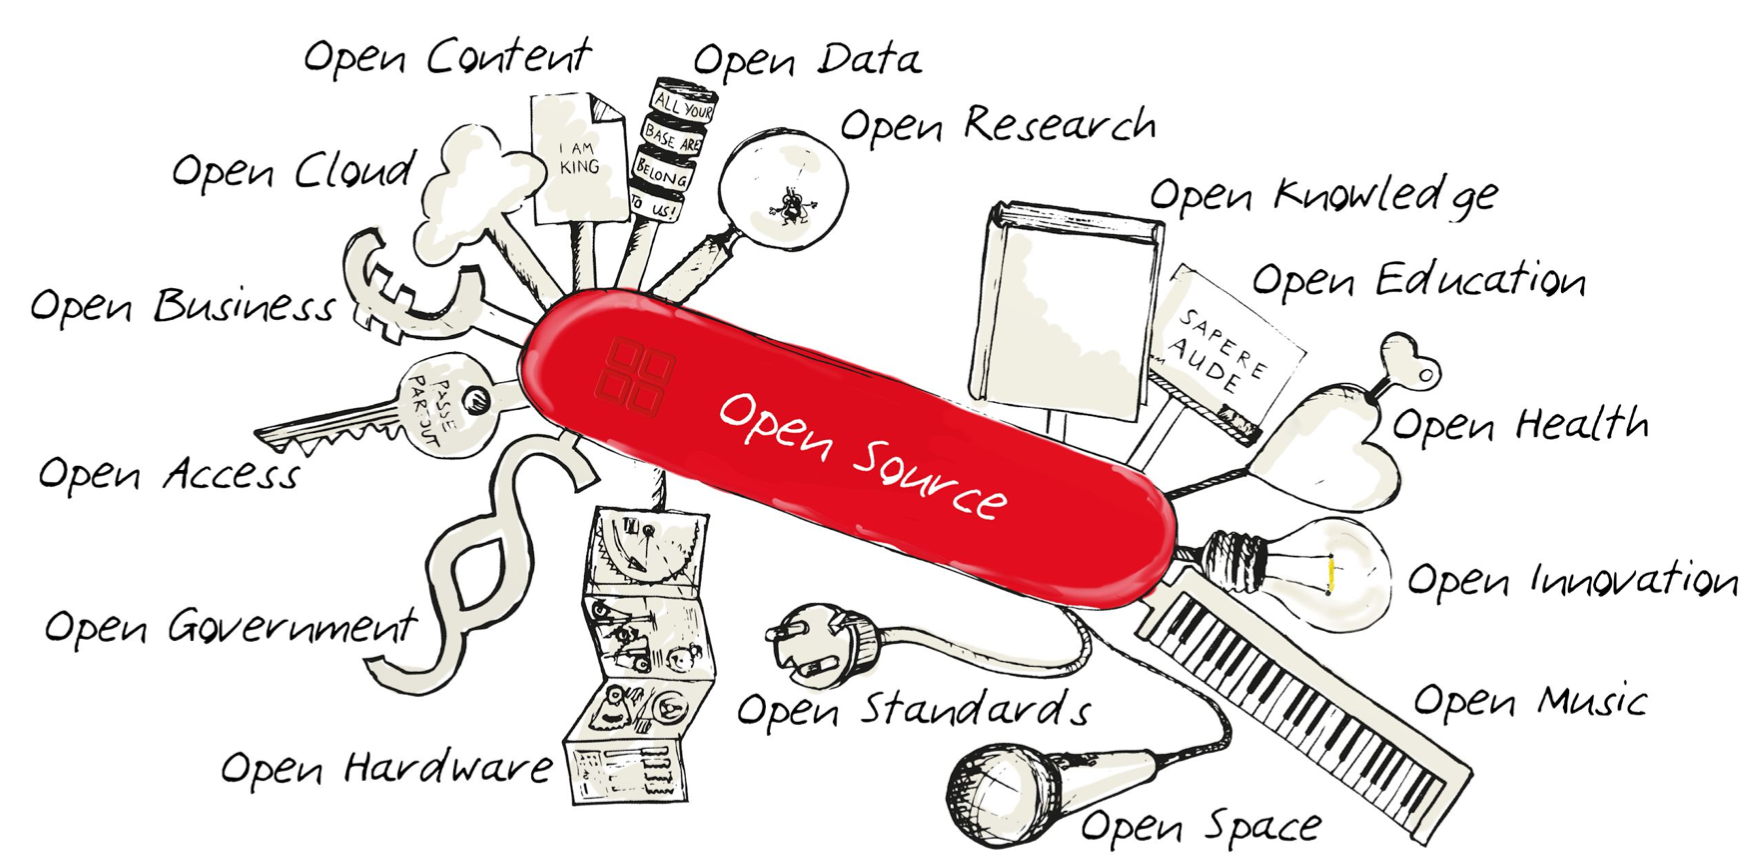
\includegraphics[width=0.8\textwidth]{assets/Open.png}
\end{figure}

\begin{itemize}
  \item Transparenz, Zusammenarbeit, Wiederverwendung, freier Zugang
  \item Daten, Wissen, Inhalt
  \item Ziel: Lösungen für viele der dringendsten Probleme der Welt
\end{itemize}

\subsubsection{Open Government}

\begin{itemize}
  \item Fokus auf Öffnung von Verwaltungsprozessen
  \item transparent, partizipativ, kollaborativ $\rightarrow$ vernetzte, aktive Bürgerschaft (Bürger einbinden, bessere Lösungen durch Wissensnutzung)
\end{itemize}

Beispiele für Initiativen

\begin{itemize}
  \item Open Knowledge Foundation Deutschland: Verbreitung von freiem und öffentlich zugängigem Wissen
  \item Offene Kommunen.NRW Institut e.V.: Offenheit, Zusammenarbeit, Transparenz auf Landes- und kommunaler Ebene
  \item Wahl-O-Mat, beteiligung.nrw.de
\end{itemize}

Open Government Partnership

\begin{itemize}
  \item gegründet 2011, 78 Staaten
  \item Regierung und Zivilgesellschaft als Partnerschaft für innovative und praktikable Lösungen
  \item \textbf{Kernkomponente: nationale Aktionspläne} $\rightarrow$ Selbstverpflichtungen und Planungen zu Gesetzesänderungen
  \item externe Evaluierung: Transparenz und Unabhängigkeit
\end{itemize}

\subsubsection{Open Data}
Zentrale Aspekte und Ziele

\begin{itemize}
  \item Fokus auf Daten und Verarbeitungsprozesse
  \item Zentrale Aspekte: Verfügbarkeit und freier Zugang, Wiederverwendung und Weitergabe
  \item Anwendung dieser Aspekte führt zu Kompatibilität und Interoperabilität
\end{itemize}

Beispiele

\begin{itemize}
  \item OpenStreetMap: offene Geodaten, ermöglicht Erstellung spezieller Karten (Wanderwege, rollstuhlgerechte Wege)
  \item Luftmesswerte: Feinstaubsensoren zum Selbstbau, zentrale Sammelstelle und Visualisierung
  \item Der Kreativität sind keine Grenzen gesetzt, ein Mehrwert z.B. durch Bereitstellung für unterschiedliche Personengruppen leicht zu erreichen
\end{itemize}

\clearpage
Herausforderungen

\begin{itemize}
  \item Spezialsoftware ohne Schnittstelle
  \item Priorisierung, welche Daten sollen bereitgestellt werden?
  \item Akzeptanz: Behörden, Ämter geben ungern Daten ab, Zeit und regelmäßiger Kontakt nötig
  \item interne Richtlinien nötig: wer, was, wann
\end{itemize}

Anforderungen

\begin{itemize}
  \item offene, lizenzfreie Formate nötig zur Interoperabilität
  \item CSV, JSON, XML, GML, GPX, ODT, ODS, ODP, TXT, HTML
  \item Metadaten in entsprechendem Format (bsp. DCAT-AP DE für Verwaltungsdaten)
  \item Freie Lizenzen: Creative Commons Lizenzen
  \item Sonderfall: Datenlizenz Deutschland für Verwaltungsdaten
\end{itemize}

\subsubsection{Ratsinformationssysteme}
Grundlagen

\begin{itemize}
  \item Informations- und Dokumentenmanagementsysteme für Parlamente
  \item Unterstützt Mandatsträger bei der Arbeit
  \item Sitzungsdienst, Workflow, Rats- und Bürgerinformationen
  \item Erfolgs- und Beschlussüberwachung
\end{itemize}

Verbindung von Open Government und Open Data

\begin{itemize}
  \item Schnittstellen zu verschiedenen Systemen (intern wie extern)
  \item Schnittstelle: OParl, Standard-API, offener Standard
  \item Unterstützung der Bereitstellung von offenen Daten (Transparenz und Teilhabe)
\end{itemize}